\chapter{El M'etodo de Separaci'on de Variables}

El m'etodo de separaci'on de variables (MSV, originalmente introducido por Daniel Bernoulli, 1700-1782) para encontrar soluciones de EDP's \textit{lineales} consiste en reducir la EDP a un conjunto de EDO's para un conjunto de funciones auxiliares. Cada una de estas funciones auxiliares depende s'olo de una de las variables independientes del problema. La soluci'on es entonces construida como una \textit{superposici'on} (e.d. combinaci'on lineal) de \textbf{soluciones separables}, consistentes en productos de las funciones auxiliares.

M'as expl'citamente, el MSV consiste en:
\begin{itemize}
\item Buscar soluciones separables de la EDP. Esto conduce a un conjunto de EDO's.
\item Construir una superposici'on general de soluciones separables, e imponer las condiciones de contorno y/o iniciales del problema.
\end{itemize}

Si bien en general el MSV sigue los pasos anteriores, en la pr'actica es 'util considerar un paso intermedio:
\begin{itemize}
\item Imponer las condiciones de contorno/iniciales homog'eneas a cada funci'on separable. Esto simplifica mucho el c'alculo puesto que t'ipicamente elimina muchas posibles contribuciones a la (futura) combinaci'on lineal. Esto s'olo puede ser realizado con las condiciones de borde/iniciales homog'eneas para EDP's lineales y homog'eneas, puesto que si la soluci'on separable satisface estas condiciones entonces cualquier superposici'on lineal lo har'a. Adem'as, no se pierde generalidad con este m'etodo, puesto que (puede demostrarse que) las funciones separables obtenidas son linealmente independientes.
\end{itemize}

En resumen, es conveniente aplicar el MSV de la siguiente forma:
\begin{itemize}
\item Buscar soluciones separables de la EDP (conjunto de EDO's).
\item Imponer las condiciones de borde/iniciales \textit{homog'eneas} a las soluciones separables.
\item Construir una combinaci'on lineal general con las soluciones separables anteriores.
\item Determinar los coeficientes de la combinaci'on lineal que aseguran que la soluci'on final satisface las \textit{condiciones de borde/iniciales inhomog'eneas}.
\end{itemize}



\section{Coordenadas Cartesianas}
\section{Ejemplo: Ecuaci'on de Laplace en dominio rectangular}
Buscaremos la soluci'on $\Psi(x,y)$ que satisface la ecuaci'on de Laplace bidimensional
\begin{equation}\label{ejLap2D}
\frac{\partial^2\Psi }{\partial x^2}+\frac{\partial^2\Psi }{\partial y^2}=0,
\end{equation}
en el rect'angulo $0<x<1$, $0<y<2$, con la condici'on de borde
\begin{equation}
\Psi(x,2) = x(1-x), 
\end{equation}
y con $\Psi=0$ en los otros tres lados. 

Primero buscamos soluciones separables de la EDP, de la forma
\begin{equation}
\Psi_{\rm sep}(x,y)=X(x)Y(y).
\end{equation}
Al reemplazar en \eqref{ejLap2D} y dividir por $\Psi_{\rm sep}$ encontramos
\begin{equation}
\frac{1}{X(x)}\frac{d^2X}{dx^2}+\frac{1}{Y(y)}\frac{d^2Y}{dy^2} = 0,
\end{equation}
lo que implica que t'ermino debe ser igual a una constante, es decir
\begin{equation}
\frac{1}{X(x)}\frac{d^2X}{dx^2} = \lambda, \qquad \frac{d^2X}{dx^2}-\lambda X(x)=0,
\end{equation}
\begin{equation}
\frac{1}{Y(y)}\frac{d^2Y}{dy^2} = -\lambda, \qquad \frac{d^2Y}{dy^2}+\lambda Y(y)=0.
\end{equation}
La forma expl'icita de estas ecuaciones depende del valor, y en particular del signo, de la constante de separaci'on $\lambda$, que por ahora tiene valor desconocido: Por ejemplo,
\begin{equation}
X_\lambda(x)= 	\begin{cases}
		c_1e^{\sqrt{\lambda}x} + c_2e^{-\sqrt{\lambda}x}, & \text{si }\lambda>0 \\
		c_1 + c_2x,  & \text{si } \lambda=0 \\
		c_1\cos(\sqrt{-\lambda}x) + c_2\sin(\sqrt{-\lambda}x), & \text{si } \lambda<0
		\end{cases}.
\end{equation}
Similarmente,
\begin{equation}
Y_\lambda(y)= 	\begin{cases}
		\bar{c}_1\cos(\sqrt{\lambda}y) + \bar{c}_2\sin(\sqrt{\lambda}y), & \text{si }\lambda>0 \\
		\bar{c}_1 + \bar{c}_2y,  & \text{si } \lambda=0 \\
		\bar{c}_1e^{\sqrt{-\lambda}y} + \bar{c}_2e^{-\sqrt{-\lambda}y}, & \text{si } \lambda<0
		\end{cases}.
\end{equation}
As'i, hemos encontrado infinitas soluciones separables, cada una de la forma
\begin{equation}\label{EjLapPsiXY}
\Psi_\lambda^{\rm sep}(x,y)=X_\lambda(x)Y_\lambda(y),
\end{equation}
para cada valor posible de la constante de separaci'on $\lambda$. Como esta constante puede tomar distintos valores, y como la EDP es \textit{lineal}, entonces cualquier combinaci'on lineal de la forma
\begin{equation}\label{EjLapPsisumaSep}
\Psi(x,y) = \sum_{\lambda}\Psi_\lambda^{\rm sep}(x,y) = \sum_{\lambda}X_\lambda(x)Y_\lambda(y),
\end{equation}
es tambi'en soluci'on.

Procedemos ahora a imponer las condiciones de borde a la soluci'on. Los c'alculos se simplifican si imponemos primero las \textit{condiciones de borde homog'eneas}. Por ejemplo, la condici'on $\Psi(0,y)=0$, $\forall y\in[0,2]$ (borde izquierdo del dominio) requiere que
\begin{equation}
\Psi(0,y) = \sum_{\lambda}\Psi_\lambda^{\rm sep}(0,y) = \sum_{\lambda}X_\lambda(0)Y_\lambda(y) = 0.
\end{equation}
La 'ultima expresi'on es una combinaci'on lineal de los coeficientes (constantes) $X_\lambda(0)$ y las funciones $Y_\lambda(y)$. Ya que las funciones $Y_\lambda(y)$ son l.i. en esta combinaci'on ser'a nula s'olo si $X_\lambda(0)=0$. An'alogamente, la condici'on 
$\Psi(1,y)=0$, $\forall y\in[0,2]$ requiere $X_\lambda(1)=0$. Estas dos condiciones sobre las funciones $X_\lambda(x)$ restringen fuertemente los valores posibles de $\lambda$. En nuestro caso particular, s'olo valores negativos de esta constante de separaci'on son permitidos. Esto ocurre si $\lambda = -n^2\pi^2$, $n=1,2,\dots$, y entonces
\begin{equation}
X_n(x)=c_n\sen\left(n\pi x\right), \qquad \lambda = -n^2\pi^2, \qquad n=1,2,\dots.
\end{equation}

Para estos valores de $\lambda$, las soluciones para $Y(y)$ son de la forma
\begin{equation}
Y_n(y) = \bar{c}_1e^{\pi ny} + \bar{c}_2e^{-\pi ny}.
\end{equation}

Imponemos ahora la condici'on de borde en la frontera inferior del dominio, es decir, $\Psi(x,0) = 0$, lo que se traduce en $Y_n(0)=0$. Esto s'olo puede ser satisfecho si $\bar{c}_1+\bar{c}_2=0$, por lo que la soluci'on se reduce a
\begin{equation}
Y_n(y) = \bar{c}_1\left(e^{\pi ny} -e^{-\pi ny}\right) = 2\bar{c}_1 \senh(\pi ny).
\end{equation}

Con esto, la soluci'on adopta la forma
\begin{equation}\label{ejLap2D2}
\Psi(x,y) = \sum_{n=0}^\infty d_n \sen\left(n\pi x\right)\senh(\pi ny),
\end{equation}
donde los coeficientes son arbitrarios. Es instructivo verificar que esta expresi'on es soluci'on de la EDP \eqref{ejLap2D}, y de las condiciones de borde homog'eneas del problema. El valor de los coeficientes $d_n$ queda determinado por la condici'on de borde no-homog'enea restante (borde superior).

Imponemos por tanto que
\begin{equation}
\Psi(x,2) = \sum_{n=0}^\infty d_n \sen\left(n\pi x\right)\senh(2\pi n) \stackrel{!}{=} f(x),
\end{equation}
con $f(x)=x(1-x)$. Esto significa que los coeficientes $d_n\senh(2\pi n)$ son los coeficientes de la expansi'on de Fourier (seno) de la funci'on $f(x)$ en el intervalo $[0,1]$. Usando las relaciones de ortogonalidad de las funciones $\senh(\pi nx)$, 
\begin{equation}
\int_0^1 \senh(\pi nx)\senh(\pi mx)\,dx = \frac{1}{2}\delta_{nm},
\end{equation}
encontramos
\begin{equation}
d_n\senh(2\pi n) = 2 \int_0^1 f(x)\senh(\pi nx)\,dx,
\end{equation}
y por lo tanto
\begin{equation}
d_n = \frac{2}{\senh(2\pi n)} \int_0^1 f(x)\senh(\pi nx)\,dx.
\end{equation}

En el ejemplo particular en que $f(x)=x(1-x)$, luego de calcular la integral correspondiente, encontramos que
\begin{equation}
d_n = \begin{cases}
	\frac{8}{\pi^3n^3}\senh(2\pi n) , & \text{para } n \text{ impar} \\
	0 , & \text{para } n \text{ par} \end{cases}
\end{equation}

Con todo esto, y denotanto $n=2k-1$, con $k=1,2,3,\cdots$, encontramos que nuestra soluci'on es dada por la siguiente serie:
\begin{equation}
\psi(x,y)=\frac{8}{\pi^3}\sum_{k=1}^{\infty}\frac{\sin[(2k-1) \pi x]}{(2k-1)^3}\frac{\sinh[(2k-1)\pi y]}{\sinh[2\pi (2k-1)]}.
\end{equation}

\begin{figure}[H]
\centering
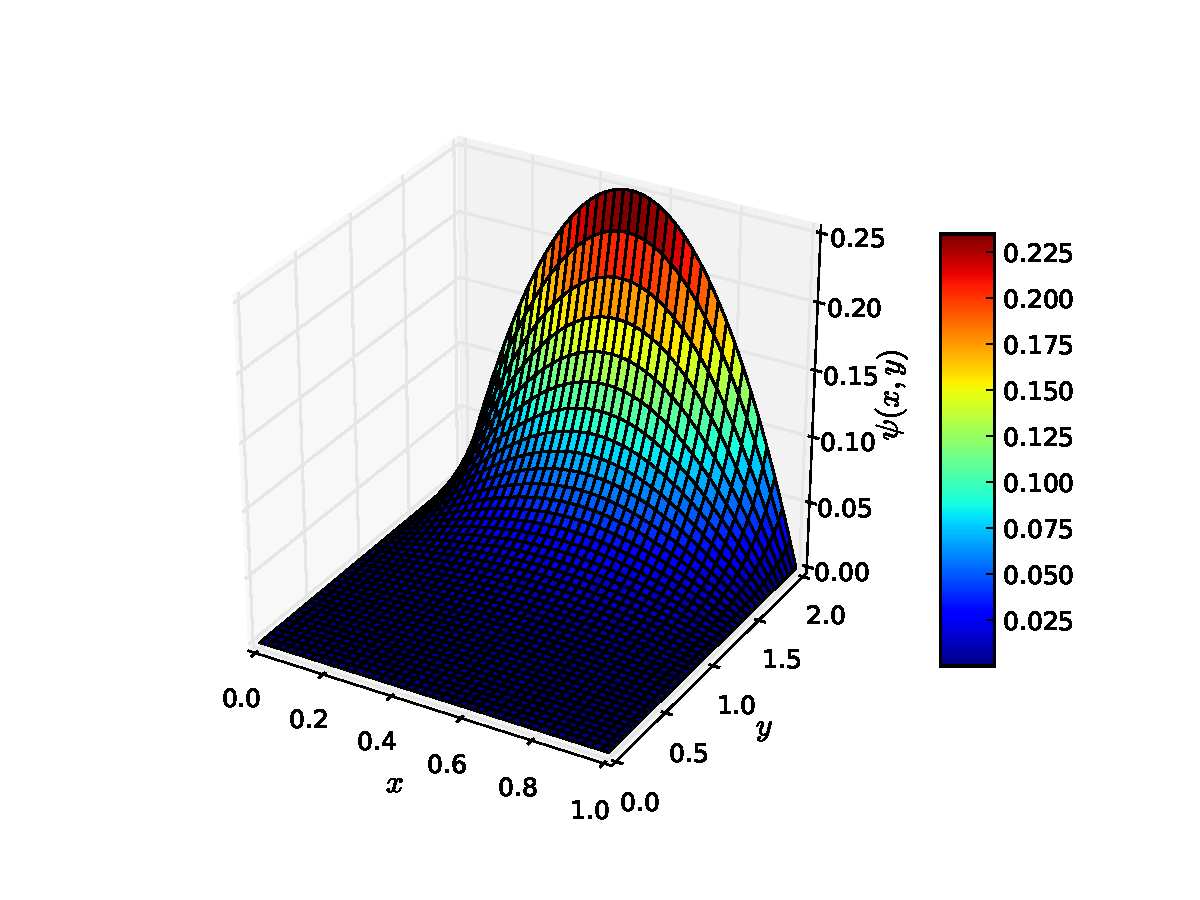
\includegraphics[angle=0,width=0.7\textwidth]{figs/fig-MSV-rectangulo-3D.pdf}
\caption{La soluci'on a nuestro problema, en 3D y colores. C'odigo Python \href{https://github.com/gfrubi/FM2/blob/master/figuras-editables/fig-MSV-Laplace-rectangulo.py}{aqu\'i}.}
\label{fig-SolLap}
\end{figure}

\subsection{Ejemplo: Ecuaci'on de onda en $1-$dimensi'on.}
Resolver la ecuaci'on de onda $1-$dimensional empleando el m'etodo de separaci'on de variables e imponiendo las siguientes condiciones de contorno 
\begin{align}
\psi(0,t)=0,\qquad \psi(L,t)=0,\label{eq:cond-borde}
\end{align}
y las siguientes condiciones iniciales 
\begin{align}
\psi(x,0)=\psi_{0}(x),\qquad \frac{\partial \psi}{dt}(x,0)=v_{0}(x),\label{eq:cond-inicial}
\end{align}
suponiendo que $\psi_{0}(x)$ y $v_{0}(x)$ son dadas pero arbitrarias de la variable $x$.

Como el problema a resolver es $1-$dimensional, la ecuaci'on a resolver es
\begin{align}
\frac{\partial^2 \psi}{\partial x^2}-\frac{1}{v^2}\frac{\partial^2 \psi}{\partial t^2}=0.\label{eq:ec-onda}
\end{align}

As'i, al emplear el MSV y suponer una soluci'on del tipo $\psi(x,t)=X(x)T(t)$, entonces
\begin{align}
\frac{\partial^2 \psi}{\partial x^2}=T(t) \frac{d^2X}{dx^2}(x),\qquad \frac{\partial^2 \psi}{\partial t^2}=X(x) \frac{d^2 T}{dt^2}(x),
\end{align}
de esta forma, al introducir las ecuaciones precedentes en \eqref{eq:ec-onda} se halla que
\begin{align}
T(t) \frac{d^2X}{dx^2}(x)-\frac{1}{v^2}X(x) \frac{d^2 T}{dt^2}(t)=0,
\end{align}
pero al dividir la ecuaci'on anterior por $\psi$, suponiendo que $\psi \neq 0$, entonces
\begin{align}
\frac{1}{X}\frac{d^2 X}{dx^2}=\frac{1}{v^2}\frac{1}{T}\frac{d^2 T}{dt^2}.\label{eq:ec-separable}
\end{align} 

Como el primer miembro de la ecuaci'on \eqref{eq:ec-separable} depende de $x$ y el segundo miembro de $t$, es evidente que ambos deben ser constantes con respecto a ambas variables, vale decir
\begin{align}
\frac{1}{X}\frac{d^2 X}{dx^2}=\lambda \text{  y  }\frac{1}{v^2}\frac{1}{T}\frac{d^2 T}{dt^2}=\lambda,
\end{align}
donde $\lambda$ es llamada la ``constante de separaci'on''. Luego podemos escribir la siguiente EDO para $X=X(x)$
\begin{align}
\frac{d^2 X}{dx^2}=\lambda X,
\end{align}
cuya soluci'on est'a condicionada por los posibles valores que tome la constante de separaci'on. Es directo verificar que
\begin{align}
X(x)=
\begin{cases}
A \cos(x\sqrt{-\lambda})+B \sin(x\sqrt{-\lambda}), & \text{si }\lambda<0\\
A' x+B', & \text{si }\lambda=0\\
A'' e^{x\sqrt{\lambda}}+B'' e^{-x\sqrt{\lambda}}, & \text{si }\lambda >0
\end{cases}.
\end{align}

Ahora bien, al imponer las condiciones de borde homog'eneas y suponer que $T(t) \neq 0$ para $t \geq 0$, entonces $X(x)$ debe satisfacer que $X(0)=0$ y $X(L)=0$. Por lo tanto
\begin{align}
A \cos(0\sqrt{-\lambda})+B \sin(0\sqrt{-\lambda})=&A \cos(L\sqrt{-\lambda})+B \sin(L\sqrt{-\lambda})=0 & \text{ si }\lambda<0,\\
A' 0+B'=&A' L+B'=0 & \text{ si }\lambda=0,\\
A'' e^{0\sqrt{\lambda}}+B'' e^{-0\sqrt{\lambda}}=&A'' e^{L\sqrt{\lambda}}+B'' e^{-L\sqrt{\lambda}}=0 & \text{ si }\lambda >0.
\end{align}

No es dif'icil verificar que el sistema de ecuaciones precedentes puede ser resuelto s'olo si $A=0$, con $\lambda < 0$ y satisfaciendo que
\begin{align}
\sqrt{-\lambda}=\frac{n\pi}{L},\qquad n=1,2,\hdots.
\end{align} 

Por lo tanto, los valores permitidos para la constante de separaci'on, tambi'en llamados ``autovalores'' o ``valores caracter'isticos'' son
\begin{align}
\lambda_{n}=-\frac{n^2 \pi^2}{L^2},\qquad n=1,2,\hdots.
\end{align}

Mientr'as que las ``autofunciones'' correspondientes est'an dadas por
\begin{align}
X_{n}(x)=B\sin\left(\frac{n \pi x}{L}\right),\qquad n=1,2,\hdots.
\end{align}

Por otro lado, la EDO para la $T_{n}(t)$ resulta ser
\begin{align}
\frac{1}{v^2}\frac{1}{T_{n}}\frac{d^2 T_{n}}{dt^2}=-\frac{n^2 \pi^2}{L^2},
\end{align}
cuya soluci'on est'a dada por
\begin{align}
T_{n}(t)=C_{n}\cos\left(\frac{n \pi vt}{L}\right)+D_{n}\sin\left(\frac{n\pi vt}{L}\right),
\end{align}
con $C_{n}$ y $D_{n}$ constantes arbitrarias. En efecto una soluci'on separable del problema es tal que
\begin{align}
\psi_{n}(x,t)=\left[C_{n}\cos\left(\frac{n \pi vt}{L}\right)+D_{n}\sin\left(\frac{n\pi vt}{L}\right) \right]B_{n}\sin\left(\frac{n \pi x}{L}\right),
\end{align}
y redefiniendo el valor de las constantes como $a_{n}:=C_{n}B_{n}$ y $b_{n}:=D_{n}B_{n}$ se encuentra que
\begin{align}
\psi_{n}(x,t)=\left[a_{n}\cos\left(\frac{n \pi v}{L}t\right)+b_{n}\sin\left(\frac{n \pi v}{L}t\right)\right] \sin\left(\frac{n\pi x}{L}\right).
\end{align}

Es directo verificar que cada una de estas soluciones satisface las condiciones de contorno homog'eneas impuestas \eqref{eq:cond-borde}. Sin embargo, ninguna de ellas, por separado satisface las condiciones iniciales \eqref{eq:cond-inicial}. Pese a ello, podemos encontrar una soluci'on al problema usando el hecho que la \eqref{eq:ec-onda} es lineal y homog'enea. Debido a esto, una superposici'on de soluciones $\psi_{n}(x,t)$, con distintos $n$, ser'a tambi'en soluci'on de la EDP. Adem'as, esta superposici'on satisface las condiciones de borde (para cualquier valor de los coeficientes que determinan la combinaci'on lineal), ya que son condiciones de borde homog'eneas.

Consideremos por tanto, una superposici'on general de todas las soluciones separables $\psi_{n}(x,t)$ disponibles
\begin{align}
\psi(x,t)=&\sum_{n=1}^{\infty}\psi_{n}(x,t)\\
=&\sum_{n=1}^{\infty}\left[a_{n}\cos\left(\frac{n \pi v}{L}t\right)+b_{n}\sin\left(\frac{n \pi v}{L}t\right)\right] \sin\left(\frac{n\pi x}{L}\right),
\end{align}
donde los coeficientes pueden ser calculados al imponer las condiciones iniciales tales que
\begin{align}
\psi_{0}(x)=&\psi(x,0)=\sum_{n=1}^{\infty}a_{n}\sin\left(\frac{n \pi x}{L}\right),\label{eq:psi0}\\
v_{0}(x)=&\frac{\partial \psi}{\partial t}(x,0)=\sum_{n=1}^{\infty}\left( \frac{n \pi v}{L}\right) b_{n}\sin\left( \frac{n \pi x}{L}\right).\label{eq:v0}
\end{align}

De esta forma, multiplicando las ecuaciones precedentes por $\sin(n\pi x/L)$ y empleando la relaci'on de ortogonalidad en \eqref{eq:ortogo-sin-cos}, se encuentra que $a_{n}$ y $b_{n}$ son tales que:
\begin{align}
a_{n}:=\frac{2}{L}\int_{0}^{L} \psi_{0}(x)\sin\left(\frac{k\pi x}{L}\right)dx \text{  y  }
b_{n}:=\frac{2}{n \pi v}\int_{0}^{L} v_{0}(x)\sin\left(\frac{k\pi x}{L}\right)dx.
\end{align}

As'i, si
\begin{align}
\psi_{0}(x)=
\begin{cases}
\frac{2A}{L}x, &\text{si }x \in (0,\frac{L}{2}),\\
2A-\frac{2A}{L}x, &\text{si}x \in (\frac{L}{2},L)
\end{cases} .
\end{align}
y $v_{0}(x)=0$, entonces
\begin{align}
a_{n}=\frac{8A}{\pi^2 n^2}
\begin{cases}
0, &\text{si }n \text{ par}\\
(-1)^{(n-1)/2}, &\text{si }n \text{ impar}
\end{cases},
\end{align}
mientr'as que $b_{n}=0$. Luego, haciendo $n:=2k+1$ con $k=0,1,\hdots$ se halla que:\footnote{En \url{http://nbviewer.ipython.org/urls/dl.dropbox.com/s/3ud8im827ntf3bw/MSV-01.ipynb?dl=0} pueden visualizar un notebook con una animaci'on de la soluci'on.}
\begin{align}
\psi(x,t)=\frac{8A}{\pi^2}\sum_{k=0}^{\infty}\frac{(-1)^k}{(2k+1)^2}\sin\left[(2k+1)\frac{\pi}{L}x\right]\cos\left[(2k+1)\frac{\pi v}{L}t\right].
\end{align}
\section{Coordenadas Cil\'indricas}
\section{Coordenadas Esf'ericas}
La ecuaci'on de Helmholtz (modificada),
\begin{equation}
\nabla^2\Psi+\alpha\Psi=0,
\end{equation}
adopta, en coordenadas esf'ericas, la forma:
\begin{equation}
\frac{1}{r^2}\frac{\partial\ }{\partial r}\left(r^2\frac{\partial\Psi}{\partial r}\right)   
+\frac{1}{r^2\sen\theta}\frac{\partial}{\partial\theta}\left(\sen\theta\frac{
\partial\Psi}{\partial\theta}\right) + \frac{1}{r^2\sen^2  \theta}
\frac{\partial^2\Psi}{\partial \varphi^2}  +\alpha\Psi= 0.\label{est20}
 \end{equation}
Buscaremos soluciones separables de la forma 
 \begin{equation}\label{produkt1}
  \Psi_{\rm sep}(r,\theta,\varphi) = R(r)\Theta(\theta)\Phi(\varphi).
 \end{equation}
 Introduciendo \eqref{produkt1} en \eqref{est20}, multiplicando por $r^2\sen^2\theta$ y dividiendo por $\Psi_{\rm sep}$, se obtiene
\begin{equation}\label{Hsep}
\sen^2\theta\left[\frac{1}{R}\frac{d\ }{dr}\left(r^2\frac{dR}{dr}\right) +
\frac{1}{\Theta\sen\theta}\frac{d\ }{d\theta}\left(\sen\theta\frac{
d\Theta}{d\theta}\right) +\alpha r^2\right]+ \frac{1}{\Phi}\frac{d^2 \Phi}{d\varphi^2} = 0.
 \end{equation}
De esta forma, podemos realizar la primera separaci'on, ya que necesariamente
\begin{eqnarray}
\frac{1}{\Phi} \frac{d^2\Phi}{d\varphi^2} = \text{const.} = -m^2. \end{eqnarray}\label{loes1}
Las soluciones univaluadas, e.d. que satisfacen la condici'on de borde per'iodica $\Phi(\varphi+2\pi)=\Phi(\varphi)$, son
\begin{equation}\label{Phim}
\Phi (\varphi) = e^{\pm im\varphi}, \qquad m=0,\pm 1,\pm 2, \cdots .
\end{equation}
Con esto, \eqref{Hsep} se reduce a
\begin{equation}
\sen^2\theta\left[\frac{1}{R}\frac{d\ }{dr}\left(r^2\frac{dR}{dr}\right) +
\frac{1}{\Theta\sen\theta}\frac{d\ }{d\theta}\left(\sen\theta\frac{
d\Theta}{d\theta}\right) +\alpha r^2\right]-m^2 = 0
 \end{equation}
que, al dividir por $\sen^2\theta$ implica que
\begin{equation}
\frac{1}{R}\frac{d\ }{dr}\left(r^2\frac{dR}{dr}\right)+\alpha r^2
+\frac{1}{\Theta\sen\theta}\frac{d\ }{d\theta}\left(\sen\theta\frac{
d\Theta}{d\theta}\right) -\frac{m^2}{\sen^2\theta} = 0.
 \end{equation}
Esta ecuaci'on est'a nuevamente separada, ya que los primeros dos t'erminos dependen s'olo de $r$ mientras que los 'ultimos dos s'olo de $\theta$. Por lo tanto, podemos introducir una segunda constante de separaci'on, $Q$, tal que las EDOS separadas se escriben como:
\begin{gather}
\frac{d\ }{dr}\left(r^2\frac{dR}{dr}\right)+\left(\alpha r^2-Q\right)R=0, \label{ecrHelmce}\\
\frac{1}{\sen\theta}\frac{d}{d\theta}\left(\sen\theta\frac{d\Theta}{d\theta}\right)
+\left(Q-\frac{m^2}{\sen^2\theta}\right) \Theta = 0. \label{ecThHelm}
\end{gather}

\subsubsection{Caso $\alpha=0$, ecuaci'on de Laplace}
 La ecuaci'on \eqref{ecrHelmce} es una ecuaci'on tipo Euler y puede ser resuelta con la
substituci'on $r:=e^t$ , $y=U(r)=U(e^t)$, o bien con el Ansatz
 \begin{equation}
  U(r) = r^l,\quad l=\text{const.}
\end{equation}
  Reemplazando esta soluci'on en la ecuaci'on encontramos la condici'on
 $l(l-1)=Q$. La soluci'on general de la ecuaci'on para $U(r)$ es entonces
\begin{equation}
 R(r) = A\cdot r^{l_1} + B\cdot r^{l_2},\label{loes2}
\end{equation}
donde $A$ y $B$ son constantes arbitrarias y $l_1$ y $l_2$ son las soluciones de la ecuaci'on cuadr'atica $l^2-l-Q=0$. Como veremos en detalle en la secci'on \ref{sec:FrobLeg}, la ecuaci'on angular \eqref{ecThHelm} s'olo tiene soluciones finitas para $\theta=0$ y $\theta=\pi$, es decir, sobre el eje $z$ si $Q=n(n+1)$, con $n=0,1,2,\cdots$. En este caso tendremos que $l_1=n$ y $l_2=-(n+1)$, y por lo tanto
\begin{equation}
R_n(r) = A_l\cdot r^n + \frac{B_n}{r^{n+1}},\label{Rn}
\end{equation}
